\documentclass[../notes.tex]{subfiles}

\pagestyle{main}
\renewcommand{\chaptermark}[1]{\markboth{\chaptername\ \thechapter\ (#1)}{}}
\setcounter{chapter}{7}

\begin{document}




\chapter{???}
\section{Machine Learning}
\begin{itemize}
    \item \marginnote{10/22:}Lecture 12 recap.
    \begin{itemize}
        \item Different electronic parameters capture different features of molecules.
        \item Electronic parameters.
        \begin{itemize}
            \item Hammett parameters ($\sigma$).
            \begin{itemize}
                \item Examples include $\sigma_p$, $\sigma_m$, $\sigma^+$, and $\sigma^-$.
            \end{itemize}
            \item Nucleophilicity and electrophilicity.
            \begin{itemize}
                \item Examples include Mayr and Swain-Scott.
            \end{itemize}
            \item NMR or IR shifts.
            \item You can also parameterize via the energy of certain electrons (e.g., $\sigma$, $\sigma^*$, lp, etc.).
        \end{itemize}
        \item Steric parameters.
        \begin{itemize}
            \item A values: Historic.
            \item Sterimol ($L$, $B_1$, and $B_5$): Common.
            \item Taft ($E_s$) and Charton for stereoelectronic.
            \item Bite angle, cone angle, and PBV for sterics in catalysis.
        \end{itemize}
        \item Why do we use parameters?
        \begin{itemize}
            \item Correlating parameters to reaction outcomes (e.g., rate, selectivity, etc.) lets us\dots
            \begin{itemize}
                \item Predict reaction outcomes;
                \item Design better catalysts;
                \item Learn something about the reaction mechanism (this is especially important for this class).
            \end{itemize}
        \end{itemize}
    \end{itemize}
    \item Announcements.
    \begin{itemize}
        \item Don't forget the exam!
        \item This is Masha's last lecture. Fill out the teaching evaluations for Masha and Jonathan at the end of the course! Masha's evals will influence her tenure decision, and Jonathan's could help win him a teaching award.
    \end{itemize}
    \item Today: More complex relationships between the input parameters from last time and our output.
    \begin{itemize}
        \item This is machine learning (ML)!
        \item Masha will focus on the applications of ML to organic chemistry, but please read more about the math and other applications if you're interested!
    \end{itemize}
    \item There will be a lot of vocab in this lecture, starting with the definition of \textbf{AI}.
    \item \textbf{Artificial intelligence}: The development of computer systems able to perform tasks that normally require human intelligence. \emph{Also known as} \textbf{AI}.
    \item Examples of such tasks.
    \begin{itemize}
        \item Speech recognition, decision making, visual perception.
        \item Not just things like calculus, but things that require a "greater" level of intelligence.
    \end{itemize}
    \item Under the umbrella of AI falls \textbf{ML}.
    \item \textbf{Machine learning}: A subfield of AI that allows computer systems to learn and adapt without explicit instructions or programming. \emph{Also known as} \textbf{ML}.
    \begin{itemize}
        \item ML is characterized by the computer system being able to do things that we didn't explicitly program it to do.
    \end{itemize}
    \item In the context of ML, we also have an explicit definition of \textbf{learning}.
    \item \textbf{Learning}: A computer program is said to form some experience ($E$) with respect to a task ($T$) and a measure of performance ($P$; aka the "performance metric"), if it's performance on $T$ --- as measured by $P$ --- improves with $E$.
    \begin{itemize}
        \item This gets into the Turing test, and what it really means to know and to learn and to be conscious. This is more the realm of philosophy, and we won't get into that.
        \item It's not like it did great from the beginning; it's that it had to get better with more experience.
    \end{itemize}
    \item Reviews on the subject of ML in chemistry.
    \begin{itemize}
        \item A great one to start for organic chemists: \textcite{bib:MLChemRev}. Four big-name corresponding authors.
        \begin{itemize}
            \item Tobias Gensch: He's new, but we'll know him soon.
            \item Sigman: The pioneer of multivariate linear regression.
            \item Doyle: First to publish ML in chemistry; her 2018 \emph{Science} paper --- \textcite{bib:DoyleML} --- exploded the field.
            \item Anslyn: Wrote our textbook; the gold standard of Phys Orgo.
        \end{itemize}
        \item Any review publsihed by Doyle or Sigman will be great to read.
        \item There are also great reviews from Connor Coley, Bill Green, and Klavs Jensen.
    \end{itemize}
    \item Types of learning: \textbf{Supervised} and \textbf{unsupervised}.
    \item \textbf{Supervised} (learning): ML that has \textbf{labeled} training data.
    \begin{itemize}
        \item This type of ML analyzes the labeled data and then makes a guess on unlabeled data. After the model guesses, we evaluate its performance.
        \item Example: Show my model 100 reactions (with their yields labeled), and then have it guess the yield of a new reaction it's never seen before.
        \item This is called "supervised" learning, because after the model guesses, \emph{we} need to show it the right answer (i.e., the label).
        \item Example: Spam filters.
        \begin{itemize}
            \item These separate spam from "ham," the technical term for good emails.
            \item We train such models by showing them a bunch of spam emails and a bunch of ham emails so that they "learn" what spam looks like.
            \item The model looks for typos, weird email addresses, requests for money, etc.
        \end{itemize}
    \end{itemize}
    \item \textbf{Labeled} (training data): A set of data in which each data point (or datum) has an input and output label.
    \item \textbf{Unsupervised} (learning): ML that has \textbf{unlabeled} training data.
    \begin{itemize}
        \item This type of ML tries to uncover relationships between data and find patterns.
        \item This is "unsupervised" because there is no right answer, no guidance, no yield.
        \item A common approach: \textbf{Clustering}.
        \item Example: Netflix recommends movies that are similar to each other (i.e., which share common actors, common runtime, common genre labels, common people who have watched them, etc.).
    \end{itemize}
    \item \textbf{Clustering}: Grouping together similar data.
    \item A really common approach is to do both of these at once in \textbf{semi-supervised} learning, our secret third option.
    \item \textbf{Semi-supervised} (learning): ML that splits data into a small labeled dataset and a big unlabeled dataset.
    \begin{itemize}
        \item We group data together and assign a label to the group.
        \item Example: Image classification, i.e., to answer the question, "which photos are of the same animal?"
        \begin{itemize}
            \item An unsupervised ML finds similar images, and then a few of those get labeled "cat," so the whole group gets labeled "cat."
            \item This is how self-driving cars and Captcha work. When you help Captcha find all the images with stairs, you're (nonconsensually) providing labels to help train image recognition models!
        \end{itemize}
    \end{itemize}
    \item We'll focus on supervised learning for the rest of today.
    \item Two types of supervised learning: \textbf{Classification} and \textbf{regression}.
    \item \textbf{Classification}: The output/label is a category.
    \begin{itemize}
        \item There are a finite number of options.
        \item Example: Photos are "cat," "dog," or "human."
    \end{itemize}
    \item \textbf{Regression}: The output/label is a continuous number.
    \begin{itemize}
        \item There are an infinite number of options.
        \item Example: We could model the cost of a house as a function of house properties (e.g., the year it was built, the year we're trying to buy it, the cost of the surrounding homes, the neighborhood school system, etc.).
        \item Example: Model $\Delta G$ as a function of reaction parameters.
        \begin{itemize}
            \item This is Hammett plots! That was linear regression, so that's why we call this, "regression."\footnote{Is there a "second time you hear it" effect in psychology that mimics ML? Unlikely to place emphasis on something the first time we hear it (e.g., Dad saying that there are crazy jobs for smart people/Maya telling me about the email tracker), but more likely when we hear it again (e.g., Carina Hong's job/Dylan Miars telling me about the email tracker). Relation to retention in learning!}
        \end{itemize}
        \item Far more common in chemistry.
        \item Formal definition: A statistical technique for determining the relationship between independent or explanatory variables ($x$) and dependent or response variables ($y$).
    \end{itemize}
    \item \textbf{Linear regression}: Describe the relationship between $x$ and $y$ as a straight line.
    \begin{itemize}
        \item Fitting to $y=mx+b$.
        \item Example: $\log(k_{\ce{X}}/k_{\ce{H}})=\rho\sigma$.
        \item Some people don't call this ML; they call this "statistics." But that distinction is really only fought over by people who care about semantics or credit. So you may hear some strong opinions in the field (e.g., Sigman doesn't call it ML), but it's just labels at the end of the day (in Masha's opinion).
    \end{itemize}
    \item \textbf{Multivariate} (linear regression): Multiple $x$ and $y$ variables.
    \begin{itemize}
        \item This is all the work of Matt Sigman, building off of his classic Hammett paper (Figure \ref{fig:multiLFER}) that we reviewed last lecture.
    \end{itemize}
    \item The ML workflow: Here are the steps if you want to go into lab and plan a project.
    \begin{enumerate}[start=0]
        \item Know or define your goal and application.
        \begin{itemize}
            \item Why do you want this model?
            \item What do you want it to do?
            \item Why do you want to use it?
            \item Why would anyone care about it?
            \item A model that can predict yield to a decimal point will need tens of thousands of data points.
            \begin{itemize}
                \item If you want a model to help you refine a ligand for a reaction that you've already studied pretty well, that's a good use.
            \end{itemize}
            \item ML is fundamentally an engineering solution, so you better have a practical use for this tool you've built.
        \end{itemize}
        \item Data collection.
        \begin{itemize}
            \item How much data?
            \item Labeled or unlabeled?
            \item Will this data come from the literature or from experiment?
            \begin{itemize}
                \item This is an especially relevant consideration in chemistry.
            \end{itemize}
            \item Be aware of bias; we, as a field, tend to overreport high-yield reactions and underreport low-yield reactions. So if we train a model based just on the literature, it will think all chemical reactions are high yield.
            \item The adage here: Garbage in = garbage out.
            \begin{itemize}
                \item If you train a model on bad data, you're going to have a bad model.
            \end{itemize}
            \item So we can go into the lab and get a bunch of low-yield reactions and feel good about it, which almost never happens!
            \item Warning: If you go to Reaxys and dump a bunch of data into a model, the error rate is 30-60\% (typos and such).
            \begin{itemize}
                \item Notoriously, the patent database used to be 60\% wrong due to bad data-scraping.
            \end{itemize}
        \end{itemize}
        \item \textbf{Parameterization}.
        \begin{itemize}
            \item Categorical descriptors (common for solvents, salts, and additives).
            \begin{itemize}
                \item Tell your model that these 10 were run in toluene, these 10 in DCM, etc. That's a common category approach.
            \end{itemize}
            \item Chemically meaningful parameters.
            \begin{itemize}
                \item This is all of last lecture: $\sigma$ values, sterimol values, etc.
                \item These are chemically meaningful because they capture a feature important to reactivity.
            \end{itemize}
            \item Graph networks: Atoms are nodes, bonds are edges, etc.
            \item Molecular fingerprints: Lists of functional groups.
            \begin{itemize}
                \item Example: My molecule contains a ketone, an ester, two methynes, etc.
            \end{itemize}
            \item SMILES, or its derivatives: This is how ChemDraw encodes molecules.
            \begin{itemize}
                \item Example: Cyclohexane is "C1CCCCC1".
                \item This string is just text, so then we can use LLMs.
                \item Masha doesn't think these work that well, but they do exist.
            \end{itemize}
            \item Most ML papers mess up by this point: They either got bad data, or misrepresented it.
            \item Most ML applications use millions or billions of datapoints, so chemistry is a bit unique in that it uses dozens of data points. How to make that tenable is a big question in both the chemistry and computer science communities!
        \end{itemize}
        \item Data preprocessing: Cleaning up the data for modeling.
        \begin{itemize}
            \item Technique: Normalization.
            \begin{itemize}
                \item Make all parameters lie in the range of 0-1.
                \begin{itemize}
                    \item To do this, just divide by the maximum value.
                \end{itemize}
                \item Example: Sterimol values of 1, 4, and 8 become 0.125, 0.5, and 1; charge values of 0.01, 0.04, and 0.08 become 0.125, 0.5, and 1.
                \item Normalization helps us make sure that the model doesn't think sterimol values are 100 times more important than charge. Essentially, it prevents bias toward parameters with large values.
            \end{itemize}
            \item Technique: Reduce the number of parameters (if needed).
            \begin{itemize}
                \item Sigman recommends 8 data points per single parameter.
                \item If we have more parameters than data points, we have an \textbf{overfit} model (see Figure \ref{fig:MLfitc}), and that is no good.
            \end{itemize}
            \item The simplest model architecture (Occam's razor) is the best model.
        \end{itemize}
        \item Data sampling: Splitting data into \textbf{training}, \textbf{validation}, and \textbf{test} sets.
        \begin{itemize}
            \item We also sometimes have an \textbf{out-of-sample} set.
            \item So we have a model, but just like in science, we need the model to make useful predictions for it to be a good model.
            \item In the validation set, the model is going to show us it's performance.
            \begin{itemize}
                \item Example: If linear regression does 70\% right and multivariate linear regression does 90\% right, we go with the multivariate architecture.
            \end{itemize}
            \item Then the performance of the model that we report is the performance on the final (test) set.
            \item Overexposing your model to the test set invalidates the model; this is called \textbf{data leakage}.
            \item Note: Chemists tend to mix up the "validation" and "test" sets in their writing.
            \begin{itemize}
                \item Just make sure that we have real evidence that the model works on \emph{unseen} data.
                \item If you see people say, "we used the validation set to test the model, and then applied the model to the test set," that's not a bad thing; that's just a semantic error.
            \end{itemize}
        \end{itemize}
        \item Training and testing: Evaluate the performance of different model architectures based on \textbf{metrics}.
        \begin{itemize}
            \item Example metrics: Accuracy, percent data explained, $R^2$, RMSE (root-mean-square error).
            \item Here, we run control and baseline models to predict the average and mode.
        \end{itemize}
        \item Interpretation and prediction: Use the trained model to predict reaction results, guide catalyst design, or present mechanistic hypotheses.
        \begin{itemize}
            \item Best practice: Test the model experimentally.
            \item Relating back to Point 0: Make sure the model is worth making.
            \begin{itemize}
                \item Make sure you use it for something cool; you don't need a chainsaw to hammer in a nail.
            \end{itemize}
        \end{itemize}
    \end{enumerate}
    \item \textbf{Parameterization}: Converting chemical information to \textbf{machine-readable} formats.
    \item \textbf{Machine-readable} (input): A number, binary value, graph representation, etc.
    \item \textbf{Training} (set): The set on which the model learns the trends.
    \begin{itemize}
        \item Roughly 70\% of the data.
    \end{itemize}
    \item \textbf{Validation} (set): The subset of the training set that help you choose between model architectures.
    \item \textbf{Test} (set): The set on which we evaluate the model performance.
    \begin{itemize}
        \item Roughly 30\% of the data.
        \begin{itemize}
            \item The actual numbers here are up to you! People do everything from $90:10$ to $60:40$.
        \end{itemize}
        \item We really only want to use the test set once or twice.
    \end{itemize}
    \item \textbf{Out-of-sample} (set): A set that helps us further validate generalizability or \textbf{extrapolation}. \emph{Also known as} \textbf{experimental validation} (set).
    \item \textbf{Data leakage}: The mixing of data between the test set and the training set. \emph{Also known as} \textbf{poor data hygeine}.
    \item \textbf{Extrapolation}: The ability to make predictions beyond the training set.
    \item Memo: Extrapolation vs. \textbf{interpolation}?
    \begin{itemize}
        \item There definitely is a difference.
        \item For an example of true extrapolation, see Sigman's paper on extrapolating a model trained on ligands with ee below 80\% to find ligands with ee beyond 80\%.
    \end{itemize}
    \item Don't report your training set performance!
    \item \textbf{Overfit} (model): A model that can predict the training set, but not new data.
    \begin{itemize}
        \item Such models cannot generalize, and they definitely cannot extrapolate.
        \item See Figure \ref{fig:MLfitc}.
    \end{itemize}
    \item There are actually three types of fitting.
    \begin{figure}[h!]
        \centering
        \begin{subfigure}[b]{0.3\linewidth}
            \centering
            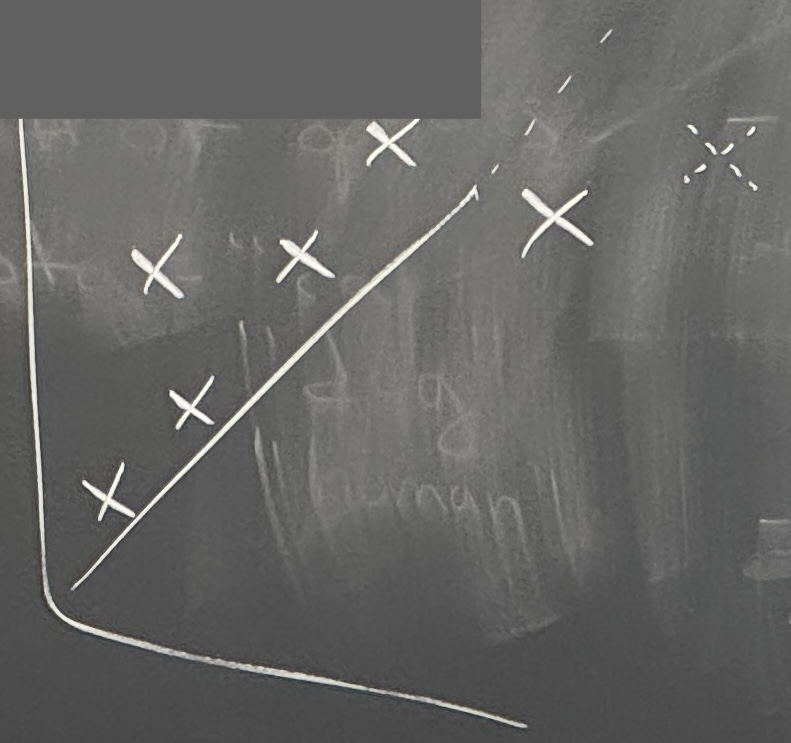
\includegraphics[width=0.63\linewidth]{MLfita.JPG}
            \caption{Underfit.}
            \label{fig:MLfita}
        \end{subfigure}
        \begin{subfigure}[b]{0.3\linewidth}
            \centering
            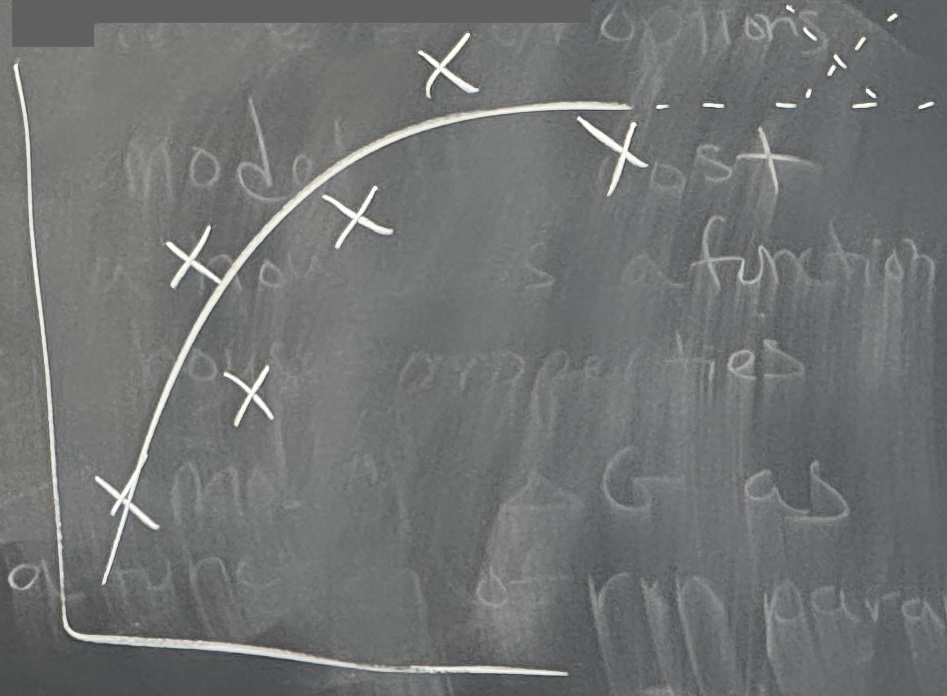
\includegraphics[width=0.8\linewidth]{MLfitb.JPG}
            \caption{Good fit.}
            \label{fig:MLfitb}
        \end{subfigure}
        \begin{subfigure}[b]{0.3\linewidth}
            \centering
            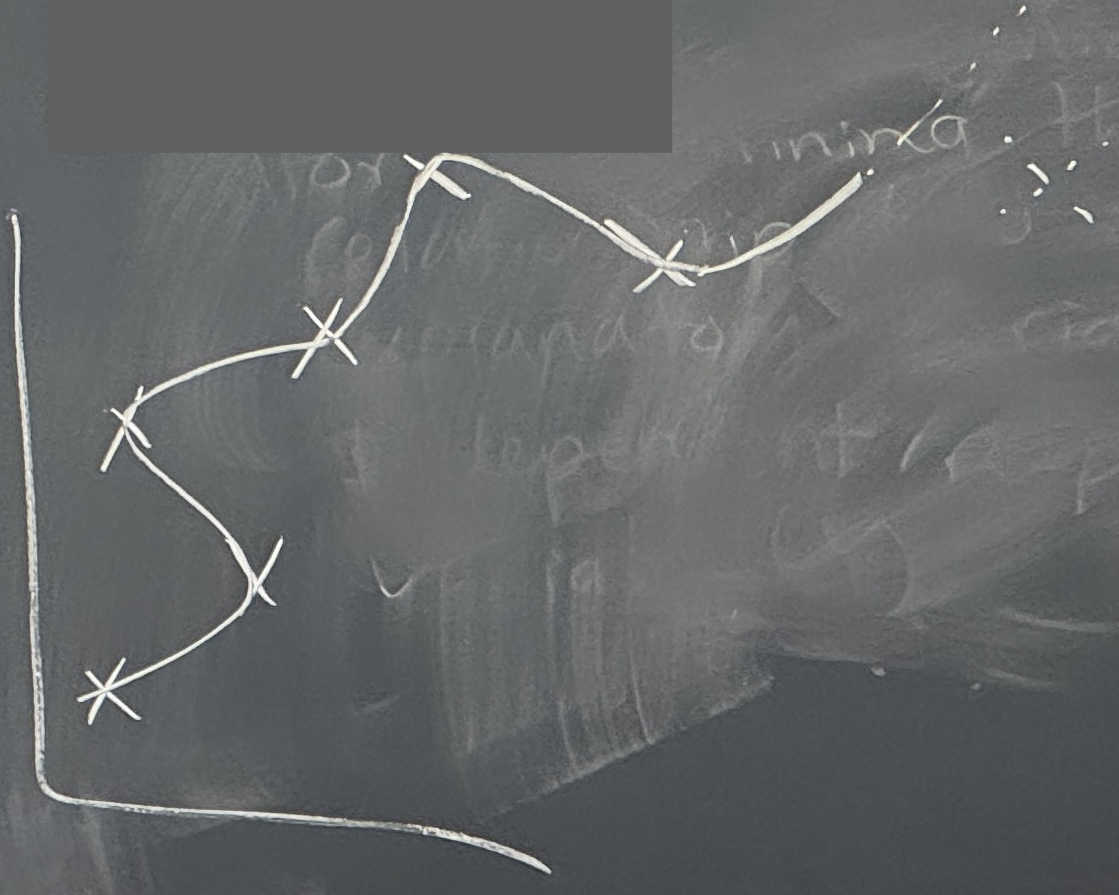
\includegraphics[width=0.74\linewidth]{MLfitc.JPG}
            \caption{Overfit.}
            \label{fig:MLfitc}
        \end{subfigure}
        \caption{Fitting machine learning models.}
        \label{fig:MLfit}
    \end{figure}
    \begin{itemize}
        \item Figure \ref{fig:MLfita}: Underfitting.
        \begin{itemize}
            \item Doesn't generalize to new data.
        \end{itemize}
        \item Figure \ref{fig:MLfitb}: Good fitting.
        \begin{itemize}
            \item Generalizes well to new data.
        \end{itemize}
        \item Figure \ref{fig:MLfitc}: Overfitting.
        \begin{itemize}
            \item Doesn't generalize at all to new data.
            \item This is tempting to chemists, because it gives them a good-looking model. But that's not actual model; that's fraud!
        \end{itemize}
    \end{itemize}
    \item Model architectures.
    \begin{figure}[h!]
        \centering
        \begin{subfigure}[b]{0.2\linewidth}
            \centering
            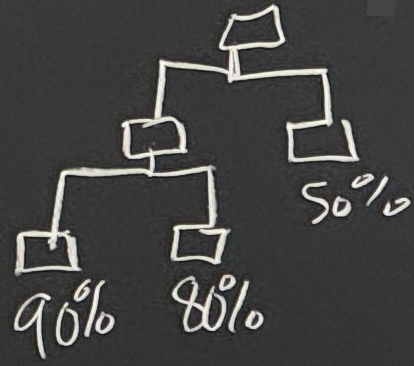
\includegraphics[width=0.8\linewidth]{MLarcha.JPG}
            \caption{Decision tree.}
            \label{fig:MLarcha}
        \end{subfigure}
        \begin{subfigure}[b]{0.2\linewidth}
            \centering
            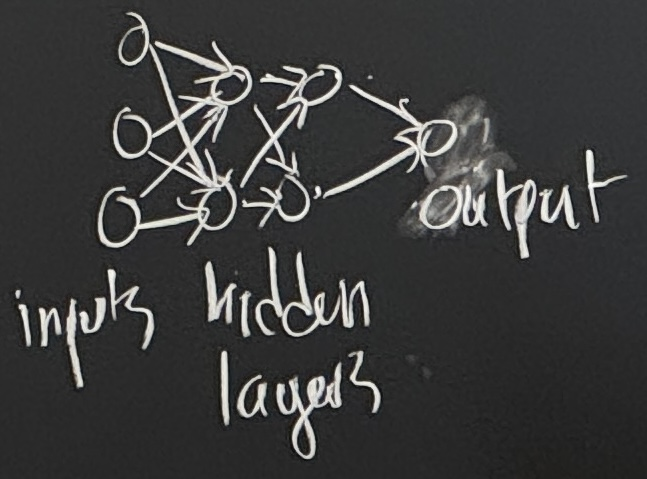
\includegraphics[width=0.9\linewidth]{MLarchb.JPG}
            \caption{Neural network.}
            \label{fig:MLarchb}
        \end{subfigure}
        \caption{Machine learning model architectures.}
        \label{fig:MLarch}
    \end{figure}
    \begin{itemize}
        \item These exist on a spectrum from models with low complexity and high interpretability to models with high complexity and low interpretability.
        \item Lowest complexity and highest interpretability: Linear regression.
        \item $k$-nearest neighbors (knn).
        \begin{itemize}
            \item Basic idea: Our ligand is close to something with high ee, so we'll probably get high ee, too.
        \end{itemize}
        \item Decision trees (Figure \ref{fig:MLarcha}).
        \begin{itemize}
            \item Answer questions such as, "high electronegativity or low electronegativity," and correlates that to ees.
        \end{itemize}
        \item Random forest.
        \begin{itemize}
            \item A subset of decision trees.
            \item Make a lot of trees and average the result.
            \item Called a "forest" because there are many trees!
        \end{itemize}
        \item Highest complexity and lowest interpretability: Neural networks (Figure \ref{fig:MLarchb}).
        \begin{itemize}
            \item Like the brain: Inputs, through hidden layers, that converge on an output.
            \item This year's physics Nobel Prize went to neural networks; Masha's not quite sure how these are physics, but they really have changed their game.
            \item They're very powerful, but extremely complex (so often overfit and not very interpretable).
            \begin{itemize}
                \item Called "black box models."
                \item Not good for mechanisms!
            \end{itemize}
        \end{itemize}
    \end{itemize}
    \item Masha also has some additional notes on model architectures that she will post on Canvas.
\end{itemize}




\end{document}